\section{Methods}

Traditional asset return predictions utilized time-series models that take into account the temporal nature of trading as sequential decision making. As such, most deep-learning applications in this area have leveraged the temporal aspect of RNN models, particularly LSTM, in making predictions (\cite{Shen2020}, \cite{Li2018}, \cite{Selvin2017}). Therefore, we use a vanilla LSTM model as the baseline model against which we compare our combined methods.

To improve upon the baseline, we introduce two additional techniques to better capture information lost in training an LSTM model. The first technique we introduce is the graph neural network (GNN) that we use to learn relational information from an implicit graph structure derived from the assets. The connectivity of the assets is evident in the log-returns correlation of the assets in our dataset as seen in figure \ref{fig:asset_corr}. This phenomenon can largely attributed to the fact that agents acting in markets tend to trade many assets at once to get better risk-adjusted returns through diversification. The interactions of these market agents with the assets determines the structure of our market graph representation. This approach is also used in \cite{Matsunaga2019}, \cite{Sun2020}, \cite{Feng2019}, and \cite{Peng2021}.

\begin{figure}[H]
	\centering
	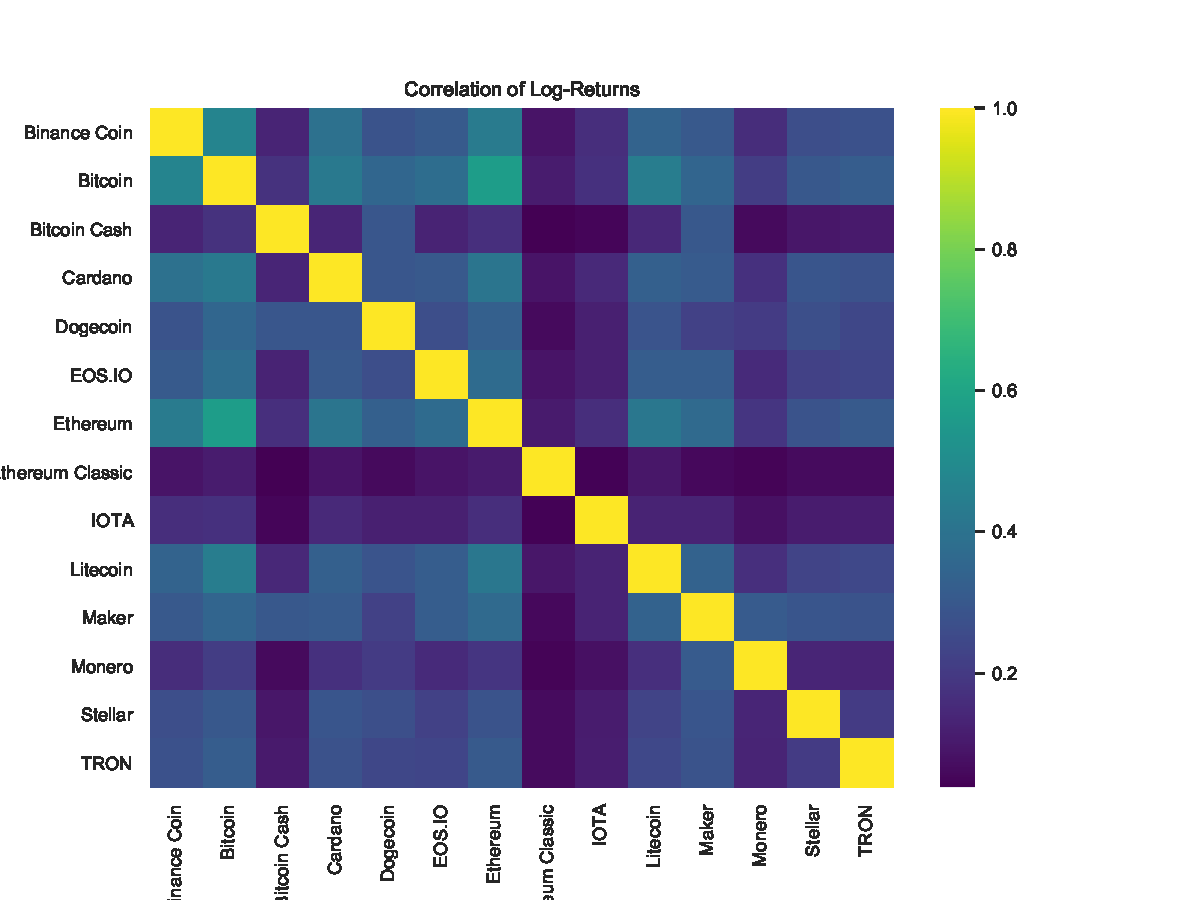
\includegraphics[width=\linewidth]{../../figures/correlation.pdf}
	\caption{Correlation of log returns calculated on minute close prices of assets. Note the high correlation among the most commonly traded assets like Bitcoin/Ethereum and Bitcoin/Binance Coin.}
	\label{fig:asset_corr}
\end{figure}

\cite{Peng2021} show empirically that using the correlation matrix as an adjacency matrix as input into GCN layers provided best performance. Therefore, we use the same, imposing a lookback window equal to the length of the sequence input to the LSTM model. Restricting this lookback window provides a basis for direct comparison as the GCN-augmented model will not have access to more information than the LSTM model and any performance boost would be a result of capturing relational information from the correlation matrix. For our specific GCN model, we implement the propogation rule taken from \cite{Kipf2017}.